\documentclass[a4paper, 11pt]{article}
\usepackage{fancyhdr}
\usepackage{titlesec}
\usepackage[margin=1.2in]{geometry}
\usepackage{url}
\usepackage{graphbox}
\usepackage{fancyhdr}
\usepackage{caption}
\usepackage{fancyvrb}
\usepackage{float}
\usepackage{pgfgantt}
\usepackage{textcomp}
\usepackage{etoolbox}
\usepackage{graphicx}


\makeatletter
%\@addtoreset{section}{part}
\makeatother

\fancypagestyle{title}{
\renewcommand{\headrulewidth}{0pt}
\fancyhf{}
\lhead{Luke Bessant - 2020}
\rhead{}}

\pagestyle{title}

\title{\textbf{CS3821 Full Unit Project Final Report}\\Computer Language Design and Engineering}

\author{Luke Bessant\\Supervisor: Reuben Rowe}

\date{\today}

\begin{document}

\maketitle

\thispagestyle{title}

\newpage

\tableofcontents
\newpage\part{Declaration}

This report has been prepared on the basis of my own work. Where other published and unpublished source materials have been used, these have been acknowledged.

\vskip3em

Word Count: 12572\underline{}

\vskip3em

Student Name: Luke Bessant

\vskip3em

Date of Submission: \date{\today}

\vskip3em

Signature:



\includegraphics{resource/Signature.png}

\newpage\part{Introduction}
\section{Abstract}
This final report on my project has the objective of explaining, justifying and criticising the work I have done over the past two terms. The project topic I chose as my first choice, and which I was allocated, was computer language design and engineering. The brunt of the work I have put into my studies over the last nearly half year has been put into this project, and will all be detailed across the parts and sections of this document. Firstly I will define the structure of this report, and then go on to begin talking about my project.

\subsection{Report Structure}
\begin{itemize}
\item{The first part of the report will outline the initial objectives and motivation with which I first started work on this project. Explained will be my aims in terms of research and implementation, and how I think carrying out this project will benefit my future career in computer science.}

\item{The third part will detail the primary professional issue involved with my project, plagiarism, and how it affected the progress of the project so far. This part will include a reflection of how I addressed the professional issue within my project.}

\item{The theory part will include all of the research reports I have written during this project, as well as a literature survey on the research materials used to obtain the knowledge necessary to write these reports.}

\item{Fifth will be a section on the software developed during this project, namely an explanation of all of the programs written, how to run them, and detailing of the software engineering methodologies used during their production.}

\item{There will then be a self-evaluation section which will review my progress over the duration of the project, and what doing a project such as this has taught me.}

\item{Finally, I will include a bibliography section indicating where any literature or other resources I have referred to during this report can be found.}

\end{itemize}

\newpage\section{Motivation}
\subsection{Problem Statement}
The original problem I set out to solve from the beginning of this project was the implementation of compiler for a JVM (Java Virtual Machine) language of my choosing. That is, a language which compiles down to Java bytecode, which can then be executed via the Java Virtual Machine. My idea was to simply represent a small subset of the original Java language.

The first steps towards this goal involved a lot of background theoretical research into how to define the grammar of a language, lexical analysis, parsing algorithms and code generation techniques. Thus the objective of this project in the first term was getting to grips with understanding the theory, and consequently ways to implement these stages in the compiler chain. 

Further objectives involved in the first term of this project were the implementation of programs which represented the theoretical research I had done to begin with. The first was to built a program demonstrating the use of context free grammars, which would simply pretty print the input grammars. This would give me a much greater understanding on defining context free grammars for programs, and use of abstract syntax trees necessary for the pretty print stage. I also had the objective of building a simple four function calculator interpreter. This would reinforce further my understanding of grammar definition, but also would be good grounds for learning how to use and simplify abstract syntax trees, then execute actions based on these. Such knowledge, I predicted, would be of great use when it came to building my final product.

The objective I set out to achieve in the second term was the implementation of the compiler previously described, using all of the relevant knowledge and expertise acquired across the first term in research and implementation.

In addition to these formal objectives which were represented in work submitted I also gave myself the objective of, over the winter break, understanding how Java \textit{.class} files are structured and how to represent high level programs in low level bytecode. This knowledge would be essential when it came to implementing the code generation stage of my compiler, due to the very strict manner in which data is organised in this low level format.

\subsection{Future Motivation}
Embarking on this project, my primary goal was to show both others and myself that I could take on a theoretically heavy topic and produce a working tool based on heavy research. I specifically picked the topic of computer language design and engineering due to my interest in language processing generally, as well as my aspiration for a career in academia; a large amount of research still goes on in this field and I chose to introduce myself to it. Consequently this project, as well as counting towards my degree, serves as an introduction into further research.

Having carried out research on aspects of the general compilation chain, I believe that I have advanced my prospects of a career in research in this field and given myself a headstart in this regard. Therefore when it comes to applying for further study on this subject, I believe my chances of success will be greater than if I based my project on web design, for example. In addition to this, the various programs I have written are further evidence of my interest and capability in this field, and will help me to carve out a career for myself in this research area.

In a more general sense, performing a project of this scale demonstrates my competence in organising and executing work at a self-dictated pace, showing self discipline, skill and resourcefulness. I believe such evidence of these qualities will be of great use when it comes to applying for a career in computer science, helping me to widen the scope of jobs available to me in both industry and academia.
 
\newpage\part{Professional Issue - Plagiarism}
\section{Description}
Professional issues are an important factor of work in computer science business, industry and academia, and it must be considered amongst professionals that their work has social and ethical consequences. Whilst carrying out this individual project on computer language design and engineering, plagiarism was most topical due to the extensive amounts of research performed by the nature of this particular field. Plagiarism is concerned with the use of resources others have produced, without correct acknowledgement or citation identifying to the reader where the resource originates from.

\section{Relevance of Plagiarism to my Project}
\subsection{Reports}
This project topic in particular requires a lot of research into algorithms and processes necessary to perform tasks such as lexical analysis, parsing and tree rewriting. Five reports were written in the first term of the project, detailed in the following parts of this report, which all required that I read into existing academic literature to make sense of the subject I was writing about. As already mentioned these reports were necessary to further my understanding of technologies relevant to my topic so that I could go on to produce proof of concept programs, and eventually a compiler. To maintain professional integrity, it was therefore necessary for me to reference the literature I had used for my research, so that credit was given where due for the resources used, and so that others who read my work would be able to find the origin of the knowledge and figures represented in my project reports.

Without correct citation the work that I had produced would have no professional standing, as the reader would not be able to verify the claims I am making about certain technologies nor criticise the resources I have used were they to be deprecated in the future. In addition to this, authors whose work I have used would not be able to formally declare that I have misrepresented the work that they had put into their resource where I have used it, without correct citation proving that theirs was the misrepresnted work in question.

In addition to this it would simply be an absolute injustice to reap the rewards of another's hard work by effectively stealing their resources. Therefore whenever I used such resources created by others in my work, either directly or as a source of knowledge, references to them were given in the bibliography section of the report in question. A good example of this, and a book that I used to insipire knowledge across all of my reports, is \textit{Compilers: Principles, Techniques, and Tools (2nd Edition)} written by Alfred V. Aho, Ravi Sethi, Jeffrey D. Ullman, and Monica S. Lam.

With all this in mind it was very important for me to properly source the materials I used during the report writing done for this individual project both for the good of myself and others. Primarily, the benefits of doing so I identify as giving of credit where necessary, and the ability for others to verify my work as a correct interpretation of the source material.

\subsection{Programs}
Throughout all but one of the programs written for this individual project, the exception being the lexer generator tool, I used the ANTLR \cite{ANTLR} parser generator to assist in my work. This allowed me to implement the parts of the programs I was interested in demonstrating, without having to worry about writing a parser for each individual product. As a parser generator usually does, this tool would take an input grammar I specified in syntax ANTLR requires and then produce a lexer and parser in Java representing the language of the grammar I passed to it. The lexer and parser I would then use in my programs to process input. This is where the plagiarism issue arises; ANTLR will generate Java code for me which I then use in my program. It is therefore right and proper for me to credit the ANTLR parser generator tool with the producting of this code, and not claim that I myself wrote it. 

Giving credit to ANTLR where it has produced code that I have used allows others who read such code to determine its origin, and therefore gives them the ability to look into using this same tool in their own work. It also allows them to visit ANTLR's documentation and learn about the sort of parsing algorithm ANTLR uses to produce its syntax parsers. Therefore supplying a reference to ANTLR gives it the publicity it deserves and helps it grow in popularity. As well as this it would simply not be ethical for me to use code generated by ANTLR and claim that it is my own; this would go against the morality and decency that any computer scientist should uphold. 

\subsection{Conclusion}
In conclusion due to the use of external materials in both my report writing and programming, plagiarism was always an issue looming over my project that I had to address or otherwise act unprofessionally and damage the integrity of my work.

\newpage\part{Theory}
\section{Interpretation}
One of the significant means of correctly executing a program written in some language is to employ an interpreter. Considering the importance of interpreters and the proposed implementation of a simple four function calculator for this project to prove the concepts of lexing, parsing and evaluation, the purpose of this section is to represent how interpreters work and aid me in constructing one.

\subsection{Interpreters}
Simply put an interpreter is a program designed to execute code written in some language by taking the code file or stream as input, and produce the desired output of said code rather than an executable program. This is done by traversing the lines of code in the input program consecutively, processing each line individually and generating their outputs one-by-one, not taking into account the larger code block around it. Thus a given line is more or less independent from those around it, other than sharing access to the same stack frame when within the same procedure, thereby having access to the variables and data models made available to other lines of code of that procedure.

Considering this procedure of running each line of a program one after the other, it can be derived that particular lines will be run more than once within certain programs. For instance the presence of a loop mandates that the code block within the loop will be run as many times as it takes until the loop terminates. This is a key inefficiency concerning interpreters and one of the reasons that interpretation is generally slower than compilation. The \textit{executable} we use to begin the running of a program written in an interpreted language is the interpreter itself, to which we pass our plaintext code.

Some examples of interpreted languages include Bash, VBScript and MATLAB. It's common that widely used languages will compile source code into an intermediate code or bytecode, which they then interpret. Languages fitting this description include Java and Python.

\subsection{The Process of Interpretation}
The first step is performing lexical analysis on the plaintext representation of the input code, written in the high level language supplied by the programmer and understood by the interpreter. The process of lexical analysis is to split the source code into a list of tokens, in other words, to \textit{tokenise} the code. This process of lexical analysis will be detailed in the next section of this report. The stream of tokens is then passed to the syntax analysis phase, detailed in section 5, which generates an \textit{abstract snytax tree}.

Following its generation the abstract syntax tree is passed to an evaluator in a structured list form, whose task is to process this list in such a way that the desired output result of the original code passed to the lexer is produced. This could be done by recursively evaluating each branch of a given tree node, perhaps the left side of the operand within a simple addition expression and then the right, and then evaluating the addition itself using the remaining left and right leaves.

\subsection{Interpretation vs. Compilation}
The processes of interpretation and compilation are structurally near-identical until the aforementioned evaluation stage after the generation of an abstract syntax tree. At this point, the interpreter goes on to directly evaluate the statements held within the tree and execute them to produce an immediate output. This makes interpreted programs easier to debug as we would be evaluating a particular line when an error occurs. Contrastingly a compiler will, from the AST, generate intermediate code in some low level language which is platform-independent. A good example of this would be the compilation process for C.

Therefore an interpreted program will usually begin execution more quickly than a program needing compilation, however due to the optimisation and code generation steps used by a compiler, the compiled program will generally be faster when running the executable file it generates. In addition, this executable will always be ready to run. An interpreted language requires the presence of an interpreter program to execute programs written using it, whereas only the executable file generated by the compiler is necessary for a given platform.

Since an interpreter relies on the presence of a plaintext source code file in its specified language, code written in an interpreted language will always have openly readable source code, unlike a compiled program consisting of byte code. Therefore we are able to keep the source code more private when using a compiled language.

%%%%%%

\clearpage
\newpage\section{Context-Free Grammar Specifications}
A context-free grammar is a language specification which allows a computer to derive the desired grammatical structure intended by the programmer to a list of tokens, from the lexical analysis phase, which make up a statement. This gives a computer the ability to understand its meaning and therefore generate the correct syntax tree for the statement which is then used in later stages of compilation or interpretation. Take for instance the following:

\begin{center}
	\textit{statement} \textbf{\textrightarrow} \texttt{while}(\textit{expression})\texttt{:} \textit{statement}
\end{center}

\noindent Represented here is a production rule for a \textit{statement}, in this example a while loop. The string on the right side is a concatenation of the keyword \textbf{while}, an opening parenthesis, a nonterminal \textit{expression}, a closing bracket, a colon, and a nonterminal \textit{statement}. We can add in the below two production rules to our grammar and assign the nonterminal 'statement' as the start symbol.

\begin{center}
	\begin{tabular}{l}
		\textit{expression} \textbf{\textrightarrow} \texttt{True} \\
		\textit{statement} \textbf{\textrightarrow} \texttt{print(}\textit{expression}\texttt{)}
	\end{tabular}
\end{center}

To allow us to generate the below string \texttt{while(True): print(True)}, belonging to the language generated by this grammar using nonterminals and terminals. \textit{Nonterminals}, terminals and production rules will be outlined in the following subsection.

\subsection{Specification}
A correctly specified context-free grammar must consist of the following components:

\begin{itemize}
	\item A set of \textit{terminal} symbols. These are characters or keywords which make up the strings of the language, e.g. \textit{[a..z]}, \textit{[0..9]} or mathematical operators. These make up the \textit{alphabet} of the language generated.

	\item A set of \textit{nonterminals} which represent the strings we can derive using their production rules. Each is the head of at least one production rule, describing the strings that can be derived from it.

	\item A list of construction rules known as \textit{productions}, defining the strings that can be created from a nonterminal. A nonterminal is \textit{head} (left side) of the production, separated by the symbol \textbf{\textrightarrow} or \textbf{::=} as ``has the form", from the \textit{body} of the production (right side), consisting of a pattern of terminals and nonterminals.

	\item Identification of the \textit{start symbol}, a nonterminal, usually the first listed or otherwise designated visually, from which we can derive all of the strings which make up the language generated by the grammar.
\end{itemize}

\subsubsection{Example}
An example for a simple two function calculator context-free grammar specification is shown below:

\begin{center}
	\begin{tabular}{l}
		\textit{operand} \textbf{\textrightarrow} \textit{operand}\texttt{+}\textit{operand} \\
		\textit{operand} \textbf{\textrightarrow} \textit{operand}\texttt{-}\textit{operand} \\
		\textit{operand} \textbf{\textrightarrow} \texttt{a}
	\end{tabular}
\end{center}

The terminals \texttt{a, -} and \texttt{+} are shown in bold, and the nonterminals are italicised. To note, we can use the ``\textbar"\ symbol to combine multiple productions with the same head into one production as below:

\begin{center}
	\begin{tabular}{l}
		\textit{operand} \textbf{\textrightarrow} \textit{operand}\texttt{+}\textit{operand} \textbar\ \textit{operand}\texttt{-}\textit{operand} \textbar\ \texttt{a}
	\end{tabular}
\end{center}

Some examples of the strings contained within the language generated by this grammar are \texttt{a, a+a, a+a-a} and \texttt{a+a+a+a}. 

\subsection{Derivations}
We \textit{derive} strings belonging to the language of a grammar by beginning with the start symbol and replacing the nonterminals in its body with the body of a production for that nonterminal, eventually ending up with a string which is an element of the language. For the grammar specified in Section 6.1 with the start symbol being our only nonterminal, \textit{operand}, we can replace this symbol with \textit{operand}\texttt{+}\textit{operand}, \textit{operand}\texttt{-}\textit{operand} or \texttt{a}.
\\\\
We show that a nonterminal $\alpha$ \textit{derives} a terminal or other nonterminal $\beta$ by $\alpha \Rightarrow \beta$. This is also called a replacement. We can show the derivation of a particular string by replacements. For example:

\begin{center}
	$operand \Rightarrow operand+operand$ $\Rightarrow \texttt{a}+operand$ $\Rightarrow \texttt{a+a}$
\end{center}

This shows the \textit{derivation} of \texttt{a+a} from \textit{operand}, proving that \texttt{a+a} is a string of the grammar from Section 6.1. During parsing we take a string of terminal symbols such as the one shown above and then try to figure out how to derive it from the start symbol.

\subsection{Backus–Naur Form Notation}
Backus–Naur form or BNF for short is simply a language for creating context-free grammar specifications, thus such specifications have near-identical structure to the previous examples of context-free grammars. Every rule in BNF takes the form:

\begin{center}
	\begin{tabular}{l}
		\textit{head} \texttt{::=} \textit{body}
	\end{tabular}
\end{center}

\noindent We can define the grammar previously defined in BNF with the following:

\begin{center}
	\texttt{operand ::= operand '+' operand \textbar\ operand '-' operand \textbar\ 'a' .}
\end{center}

\noindent The example shown above also defines a \textit{recursive statement} since the production rule makes use of the head nonterminal in its body. We can also surround certain contents of the body of a BNF production in curly braces to indicate zero or more repetitions of the contents. For example, when specifying functions which take a list of parameters we can use \texttt{\{<parameter>\}} within the body to indicate zero or more parameters. In conclusion, the use of BNF is to give us a standard syntactic structure for specifying context-free grammars.

%%%%%%

\clearpage
\newpage\section{Lexical Analysis}
As the first stage in the compiler toolchain, lexical analysis takes the raw source code of a program written in a language supported by the compiler and processes it in such a way that the program is split up into \textit{lexemes}, which by their character pattern are identified as particular \textit{tokens}, and then passed to the parser for syntax analysis. Lexemes are sequences of characters which match the pattern for a particular component of the programming language supported by the compiler. These lexemes represent the individual parts which make up a statement or expression within a program. Take the expression below:

\begin{center}
	\texttt{sum = sum + 50}
\end{center}

\noindent We can split this expression into the lexemes \texttt{sum}, \texttt{=}, \texttt{sum}, \texttt{+} and \texttt{50}, and are able to tell that this simply adds 50 to the current value of \texttt{sum} and reassigns the result as \texttt{sum}. Since the lexical analyser simply takes the stream of characters from our source program, it has to create lexemes from a sequence of consecutive characters using the production rules for tokens outlined within the grammar for the language. This stream of tokens is then sent to the next stage, syntax analysis to be structured.

\subsection{Tokens}
A token is a pair of the form \textlangle{}\textit{token-name, token-attribute}\textrangle{} denoting the type and contents of a valid lexeme. Many lexemes can match the pattern for a token, therefore we have the option to use an attribute for the token to give the compiler more information about it. This could be a literal value or a pointer to a position in the program's \textit{symbol table}. Upon discovering a pattern matching a valid token, the lexeme is identified by the lexical analyser as an instance of that token. 

For example, the lexeme \texttt{50} in the above expression could be recognised as an \texttt{integer} token and thus the lexer will create the token \textlangle{}\texttt{integer, 50}\textrangle{}. The lexeme \texttt{sum} could match the pattern of an \textit{identifier}, in which case a possible token could take the form \textlangle{}\texttt{id, 1}\textrangle{}. Here \texttt{id} is shorthand for identifier, and \texttt{1} is a pointer to a location within the program's symbol table where more information about the identifier is held, such as the identifier's name, type and current value. Some of the common token types across programming languages are as follows:

\begin{itemize}
\item A token for all identifiers within the language.
\item A token for the keywords within a language, such as \texttt{if} and \texttt{else}.
\item One token for all mathematical and boolean operators, or one for each individually.
\item Tokens for literal strings and types of numbers supported by the language.
\item Tokens for punctuation symbols such as brackets, commas and semi-colons.
\item A token for whitespace, which is usually not passed to syntax analysis but is instead omitted by the lexer.
\end{itemize}

\subsubsection{Attributes of Tokens}
In cases where many lexemes match the pattern of a token, we need to pass more information about the lexeme to the parser so the correct incantation can be properly reproduced in the code generation phase of the toolchain. The name/type of the token is used within the parser to make decisions about program structure, whereas the attribute value is used later on when translating tokens during code generation. From the above example, we have \textlangle{}\texttt{integer, 50}\textrangle{}.

For the identifiers of a program we need to encompass several pieces of information within one token, such as the name, type and current value of the identifier. In these cases the token attribute would point to an entry in the program symbol table where this information is held. As we saw from the previous section, an example of this is \textlangle{}\texttt{id, 1}\textrangle{} where \texttt{1} represents row one within the symbol table.

For keywords and operations of which the raw characters of the lexeme match the token name, we can simply omit the attribute and use only the token name within the token. An example of this could be \texttt{if}, where we can discard the attribute value, which matches the token name, and simply use the token \textlangle{}\texttt{if}\textrangle{}.

\subsubsection{Recognition of Tokens}
Using finite-state automata we can model each of the production rules for the tokens of our grammar by converting their regular expression to a set of states with transitions between them, a transition for each of the potential letters the expression should recognise. For instance we have the following finite-state automaton for a production \texttt{id} \textbf{\textrightarrow} \texttt{letter(letter|digit)*}:

\begin{figure}[H]
	\centering
	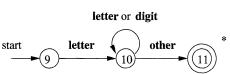
\includegraphics[width=60mm]{resource/FA.png}
	\caption{Finite-state automaton for \texttt{id} (figure 3.14 from \textit{Aho - Compilers - Principles, Techniques, and Tools - page 132)} \label{overflow}}
\end{figure}


\noindent This accepts only patterns beginning with at least one letter, and then allowing any number of letters or numbers following this. If we read a character which is not a letter or digit, then we know that this is not part of the identifier comprised of the previous characters, so we can move to the accepting state. The asterisk atop the accepting state signifies that the last character of the lexeme (\textbf{other}) is not a valid member of the pattern for this token and so the \textit{forward pointer} of the scanner is retracted by one character so as to point to the last character of the identifier. We can determine that any sequence of characters leading to the accept state of this finite-state automaton, except the \textbf{other} character, makes up an identifier as defined by our grammar.

%%%%%%

\clearpage
\newpage\section{Sentential Derivations and Top-down Parsing}
The syntax analysis phase within the compilation chain involves taking the stream of tokens derived from some source code using lexical analysis, and organising them into a syntax tree which represents the grammatical structure intended by the writer of the source code. This section will describe how to derive an input string belonging to the language of the grammar in use from its the start symbol, the construction of syntax trees from such derivations and the key aspects of the top-down parsing method.

\subsubsection{Syntax trees}
The syntax tree shown below, with accompanying grammar, gives an example tree structure for an expression \texttt{id + id * id}, where the operators are separate tokens with each \texttt{id} being an identifier.

\begin{figure}[ht!]
	\centering
	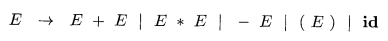
\includegraphics[width=90mm]{resource/GrammarExample.png}
	{\caption*{(4.7): \textit{Aho - Compilers - Principles, Techniques, and Tools - page 222}} \label{overflow}}
\end{figure}

\begin{figure}[ht!]
	\centering
	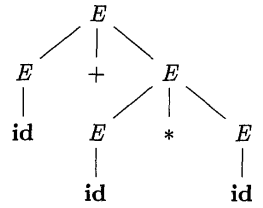
\includegraphics[width=40mm]{resource/SyntaxTree.png}
	{\caption*{Figure 4.5: \textit{Aho - Compilers - Principles, Techniques, and Tools - page 204}} 
	\label{overflow}}
\end{figure}

From this simple tree we can see that we must add to the leftmost \texttt{id} the result of the rightmost subtree of the root node (\texttt{id * id}), the start symbol of our grammar, \texttt{E}. Each inner node is is a production of our grammar and each leaf is either a terminal or nonterminal.

\subsection{Derivations}
The stream of tokens received from the lexer allows us to derive the structure of the tree corresponding to a clause, and the contents of the leaves by rewriting rules starting from the starting symbol (\texttt{E} in figure 4.5). Such rewriting involves taking some nonterminal and replacing it with the body of one of the productions for which that nonterminal is the head. By the grammar shown in (4.7), we can make the following derivation steps: 
\begin{center}
$\texttt{E} \Rightarrow \texttt{E+E} \Rightarrow \texttt{E+E*E} \Rightarrow \texttt{id+E*E} \Rightarrow \texttt{id+id*E} \Rightarrow \texttt{id+id*id}$
\end{center}
We say that \texttt{E} \textit{"derives"} \texttt{id+id*id}, proving that \texttt{id+id*id} belongs to the language generated by the grammar, that it is a \textit{sentence} of the language. Sentences which can be derived from the start symbol are \textit{sentential forms} of the grammar. If we can derive a string $\alpha$ from a start symbol \textit{S} in some sequence of zero or more derivation steps then $\alpha$ is a sentential form of the grammar.

At each step in the derivation we have a choice of which nonterminal to replace, and which production with that nonterminal as a head to replace it with. A \textit{leftmost} derivation is one where we always pick the leftmost nonterminal of the current sentence to replace. The alternative is \textit{rightmost} derivation.

\subsubsection{Parse tree derivation}
Parse trees allow us to represent the grammatical structure of a sentence at any given step in the derivation sequence. Assume our current syntax tree consists of merely the start symbol \texttt{E}. By applying the derivation $\texttt{E} \Rightarrow \texttt{E+E}$ we simply add three child nodes to our current root node \texttt{E}; \texttt{E}, \texttt{+} and \texttt{E}, shown below.

\begin{figure}[ht!]
	\centering
	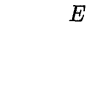
\includegraphics[align=c,width=16mm]{resource/SyntaxTree2.png}
	$\Rightarrow$
	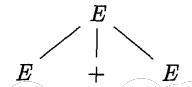
\includegraphics[align=c,width=30mm]{resource/SyntaxTree3.png}
\end{figure}

\noindent We can then continue to replace nonterminal leaves in this syntax tree with production bodies until left with the tree shown in figure 4.5, which represents the sentential form \texttt{id+id*id}. This, as well as the derivations mentioned previously, are characteristic of a \textit{top-down} and \textit{leftmost} approach to parsing. Namely, we construct a syntax tree from the root and select the leftmost nonterminal to replace at each step in the derivation sequence.

\subsection{Top-down parsing}
Top-down parsing involves constructing a syntax tree starting from the root and working down towards the leaves, creating the nodes of the tree in preorder form. This implies that we find the leftmost derivation of the input string. Thus we have the problem of deciding which production to apply to the leftmost nonterminal. We then try to match the terminal symbols in the body of the production with those of the input string. There is a possibility of selecting an incorrect production meaning we cannot then match the input, we can \textit{backtrack}, or otherwise proactively prevent the selection of an incorrect production by \textit{predictive parsing}.

\textbf{Backtracking}: When it is identified that for all possible productions for a nonterminal $\beta$ within a production body for another nonterminal $\alpha$, there is no production which leads to a correct matching of the input string, we simply backtrack to $\alpha$ and choose another possible production. If no tree can be constructed by rewriting nonterminals from the root, which represents the input string, then this string does not belong to the language generated by the grammar used.

\textbf{Predictive parsing}: To eliminate the necessity of backtracking, we can implement a lookahead. We consider the next \textit{k} symbols $a_1, ..., a_k$ within the token stream when selecting a production to replace a nonterminal \textit{A} with. Usually this lookahead is simply one symbol. In this case, we select the production for which the first terminal matches $a_{1}$, the next symbol. This holds so long as there is no left-recursion within the grammar used and it is left-factored. We select a production $\textit{A}\rightarrow\alpha$ if the next symbol $a_1$ is in the set of terminals that begin strings derived from $\alpha$. The \textit{LL(k)} class of grammars is the for one which we can construct predictive parsers with a lookahead of \textit{k}. The first \textit{L} denotes that the input strings are read from left to right, the second \textit{L} denotes that we carry out leftmost derivation, and \textit{k} is the lookahead we use.

\subsubsection{Recursive descent parsing}
This method of parsing involves the use of a set of procedures for each nonterminal within the grammar, with the procedure for the start symbol being the first called. If this procedure halts without error then we would have scanned the entire input string. Within each nonterminal's procedure, we select a production to replace the nonterminal with and scan its body. For each symbol $X_1X_2...X_k$ in the body, if $X_i$ is a nonterminal we call its corresponding procedure, otherwise if $X_i$ equals the next input symbol in the string we advance to the next symbol, else the production selected cannot match the remaining input string, so we throw an error.

The selection of the production rule to use within this procedure could be based on the backtracking heuristic, i.e. we could loop over and try all possible productions for the nonterminal until success or when no more productions exist. In this case if the application of one of the productions results in failure, we can simply try another. An error is then thrown when none of the productions for the nonterminal support the input string, in which case we go back to the procedure which called the current one.

Alternatively we could use the predictive parsing method, looking a symbol ahead to help us select the correct production with which to replace a nonterminal. In this case we report failure and return immediately when $X_i$ is not a nonterminal, nor the next terminal in the input string.

\newpage\section{Literature Survey}
\subsection{Existing Systems}

\subsubsection{OpenJDK\cite{OpenJDK}}
OpenJDK's \textit{javac} is the Java compiler tool I use on my system, with each JDK (Java Development Kit) version being an implementation of the Java language specification for Java versions 6 through 13 currently, the version I use being OpenJDK 13. Unlike the compiler I have implemented, this compiler supports the entire Java language, whereas my own supports only a small subset. Similar to my own compiler, however, \textit{javac} is written in the Java programming language. One can, with OpenJDK installed on their system, compile a Java program by running ``\texttt{javac /path/to/file.java}" on *nix systems. This compiler seems to work very well and I myself have never experienced any problems with incorrect logic or bugs, providing fully detailed information on things like exceptions and errors where they appear in my code. Therefore this tool is a very good example to take note of when writing implementing a Java compiler.

\subsection{The GNU Compiler for Java\cite{GCJ}}
The GCJ is a ``free software" implementation of the Java language, and is a part of the GCC (GNU Compiler Collection). This compiler is able to compile Java source code down to both Java bytecode, as well as native machine code. The documentation for this compiler claims that Java AWT and Swing are not currently supported, however ``most" other features are. Once installed, one is able to  comiple to native machine code by using the \texttt{-c} flag as in \texttt{gcj -c HelloWorld.java} which will compile to \texttt{HelloWorld.o}, or to a Java class file with \texttt{gcj -C HelloWorld.java}. Unlike OpenJDK's \textit{javac}, GCJ is written in C and therefore can be said to be faster that OpenJDK's implementation. Similarly the ability to compile down to machine code also means that running the produced program will also produce faster results, due to there being no need for the JVM to interpret any Java bytecode.

\subsection{Sources of Information}
\subsubsection{Compilers - Principles, Techniques, and Tools \cite{Dragon}}
This book has been the basis of the vast majority of my research, covering all of the research topics necessary to become an expert in this field. The only research topic not covered within this book being interpretation as its own part with a comparison to compilation. However the components of interpreters such as lexical and syntax analysis are of course detailed in their own chapters. Detailed explanations and examples are provided in this book for all of the technologies relevant to my final submission project, and therefore also helped me with research in this regard. In conclusion this book has been extremely useful in its detailed explanation of all of the topics under the umbrella subject of compilers. Therefore I would recommend this book as the primary material to learn all of the topics in this report, other than interpreters.

\subsubsection{Introduction to Compiler Design \cite{ItCD}}
This is another book covering of the standard topics within the field of software language engineering. This is a shorter read than \textit{Compilers - Principles, Techniques, and Tools} and was therefore at times much more helpful when I needed to quickly discover the theoretical basis behind some technology I was implementing. For example, this book contains a very well detailed section on type checking which was fundamental to my understanding of how to myself implement this stage of the compiler chain. Interesting and well thought out explanations of all topics covered allowed me, the novice, to understand all of the methodologies necessary for my own compiler implementation. I would strongly recommend this book as a first introduction to the field of compilers from my own experience.

\subsubsection{Writing Hello World in Java Byte Code\cite{HelloWorld}}
As a first introduction to Java byte code, this blog post was very instructive and taught me a lot about how how one goes about formatting a \textit{class} file so that it can be recognised and run by the Java Virtual Machine. The article takes the user step by step through what is required in terms of byte code for the user to write a program which prints \textit{Hello World}, detailing all the necessary components such as the constant pool and method attributes. This simple guide made it very easy for me to learn some simple byte code, but also introduced me to the format and structure needed by \textit{.class} files. This blog post could only be improved by also including how to write byte code for class constructors. Despite a \textit{"Hello World!"} Java program not needing a constuctor since no \texttt{Main} objects are ever initialised, it would still be helpful to detail how to implement these, since the \textit{javac} compiler by default builds constructors for all user-defined classes. 

\subsubsection{Java Code to Byte Code\cite{JavaToByteCode}}
Another very useful blog post about code generation, this post went into detail on how to represent variables and control flow in Java byte code. Detailed descriptions of each byte code operation used, as well as diagrams showing what the stack looks like at each step of a series of operations are present on this page. This made it very easy for me to get to grips with implementing essential features such as variable declaration, initialisation and \textit{if} statements in byte code. One downside is that the post specifies future articles on more essential syntax such as use of the \textit{new} keyword for object/array initialisation and method calls, however these haven't yet been written. Further components of the Java language which I did not implement, such as \textit{switch} statements were also present. To conclude, this was a very useful and informative read which I would recommend to anyone trying to understand byte code representation of control flow statements. 

\subsubsection{The Java Class File Format\cite{ClassFile}}
This is Oracle's own documentation of the format of \textit{class} files recognised by the Java Virtual Machine. Including specification of how many bytes the JVM is expecting for all of the information required, and how to format information such as constant pool entries, fields, methods and attributes, this documentation was very useful as a reference when generating the bytes for my own \textit{class} files. Reading this documentation is essential for anyone who wants to implement their own Java byte code compiler, since this is where all of the information necessary to learn how to format files recognisable by the Java Virtual Machine is. The documentation is very comprehensive but every component is easy to understand by looking at the structured descriptions in the sections with pale yellow background.

\subsubsection{Crafting Interpreters \cite{Crafting Interpreters}}
In terms of learning the background theory of interpreters, this website was a key asset. This website provides easy to understand explanations of how interpreters work, as well as giving a comparison of the difference between interpreters and compilers. The website's purpose is to show one how to implement a byte code interpreter, but it was also useful in that I was able to learn a good amount of information about how interpreters work from it.

\subsection{Conclusion}
All of the material used for research during the duration of this project was very useful and allowed me to develop the understanding in the field necesary to build a working compiler. The blog posts mentioned as sections 9.2.3 and 9.2.4 were necessary due to my lack of understanding of code generation. Therefore if I were to conduct such a project again, I would read more into the code generation sections of the compiler books mentioned in 9.2.1 and 9.2.2, which would also allow me to better understand topics such as code optimisation. To conclude therefore, I would allow myself more time across the project to read into all of the sections of each of these books which cover material essential for implementing a compiler.

\newpage\part{Software}
All of the following programs merely require a Java version of 6 or higher to run. An example of the running of each program in a Linux environment is given, however one will be able to run each program from a Windows or MacOS environment with similar commands. 

\section{Proof of Concept Programs}
This section of the report lists the proof of concept programs written during the first term of this project; the purpose and context of each program, how it was built, how it was tested and the problems involved in its construction.

For all the programs to be described, a demonstration of each is shown in the following video \texttt{https://www.youtube.com/watch?v=gE9WznhKO1g}

\subsection{BNF Pretty Printer}
The first proof of concept program written was one which is able to take in a grammar written in extended-BNF format from a file and pretty print it, making it easier to read. This program was first proposed with the idea that it would allow me to gain experience in using abstract syntax trees. Whilst this was the case. I would also say that a large portion of the benefit of working on this program was learning how to write a context-free grammar.

The ANTLR parser generator was used in the making of this program, with which we could write a grammar which recognises other EBNF grammars. This grammar supports grouping of production clauses, optional clauses, kleene and positive closures, as well as empty productions. Upon the passing of a file containing the EBNF grammar to the program, the ANTLR parser generator is used to generate an abstract syntax tree containing the structure of the productions within the file. We can then recursively handle each sub-tree, corresponding to a single production rule, whose contents we can properly format by trimming whitespace and creating a new line for alternations.

\begin{figure}[H]
\centering
\begin{BVerbatim}
start ::= '[' digit_list ']' .
digit_list ::= digit digit_tail . 
digit_tail ::= # 
	| ',' digit_list . 
digit ::= '0' 
	| '1' 
	| ( '2' | 'two' ) 
	| '3' 
	| '4' .
\end{BVerbatim}
\caption{Example pretty printed grammar output}
\end{figure}

No meaningful problems were encountered during the building of this program, the only research being into how the syntax trees generated by ANTLR are formatted. Test-driven development with JUnit test suites was used to ensure that the program could be built without any bugs which could otherwise have been introduced.
\subsubsection{Running}
Steps to download and run the BNF pretty printer on Linux systems:
\begin{verbatim}
git clone https://github.com/RHUL-CS-Projects/FullUnit_1920_LukeBessant
cd FullUnit_1920_LukeBessant/BNF\ Pretty\ Printer/bin
java -jar BNF\ Pretty\ Printer.jar /path/to/grammar.bnf
\end{verbatim}

\subsection{Stack Code Interpreter}
The purpose of this program was to make a simple four function calculator, demonstrating the ability to use abstract syntax trees and the understanding of interpretation. As well as this, the program was written in such a way that we also perform some simple code generation. Namely, the expression the user inputs is converted to a stack code format (shown below) which is then interpreted by the program to produce the desired result. This program uses the type Double for both inputs and outputs, allowing for necessary precision.

\begin{figure}[H]
\centering
\begin{BVerbatim}
PUSH 10.0;
PUSH 5.0;
ADD;
PUSH 2.0;
DIV;
PUSH 2.5;
MUL;
\end{BVerbatim}
\caption{Example stack code for expression (10+5)/2*2.5}
\end{figure}

\noindent A grammar was written which supports infix expressons using addition, subtraction, multiplication and addition, for which a parser was generated using ANTLR. I then implemented a class with which we reduce the syntax tree to make it easier to convert to stack code. This reduced tree is then traversed with a post-order search, allowing us to push the left and right sub-expressions of an operation it itself is performed, as shown above where we push \texttt{10.0} and \texttt{5.0} before adding them. A grammar was then written which recognises this stack code, so that we can interpret it and calculate the result of the original expression. 

JUnit testing was used in the making of this program to reduce the likelihood of bugs being introduced. There were no major learning curves to note, where, as before, the only research necessary was into the formatting of trees generated by ANTLR which we then have to traverse. 
\subsubsection{Running}
Steps to download and run the calculator interpreter on Linux systems: Using JAR file:
\begin{verbatim}
git clone https://github.com/RHUL-CS-Projects/FullUnit_1920_LukeBessant
cd FullUnit_1920_LukeBessant/Calculator\ Interpreter/bin
java -jar Calculator\ Interpreter.jar
\end{verbatim}
This will open up a prompt in which the user can simply type expressions.

\subsection{Lexer Generator}
The third proof of concept program involved writing a program that could recognise and write the automata necessary to support user inputs given some regular expression. Thus the idea was to write something that could, given some extension, assign user inputs a token based on a set of regular expressions. Currently the program takes one regular expression as an argument when it is run, builds the automata which recognise it and then poll the user for strings, outputting for each whether the automaton reaches an accepting state at the end of the string.

The aim is to generate the most minimal deterministic finite-state automaton with the least number of states possible, as this will be the most efficient tool with which to accept or reject a string. To do this, the input regular expression is first expanded into a format which Thompson's construction can understand, e.g. \texttt{[a-b][a-bA-B0-1]*} is converted to \texttt{(a|b)(a|b|A|B|0|1)*}. We then perform Thompson's construction with this expression. However for large expressions Thompson's construction gives us a large number of states, much more than is necessary, which will slow down the generation of a deterministic finite-state automaton when using the powerset construction, an $O(2^n)$ algorithm where $n$ is the number of states the input nondeterministic finite-state automaton has.

With this in mind when performing Thompson's construction, we minimise the automaton generated by each recursive step of the construction before returning it. For instance with the regular expression \texttt{(a|(b|c))*}, we first create the NFA for \texttt{(b|c)}, then perform the powerset construction to generate the DFA for this, then hopcroft's algorithm to convert this to the minimal DFA. We then do the same for \texttt{a|(b|c)}, and for \texttt{(a|(b|c))*}. We then run the final NFA from this construction through the powerset construction and Hopcroft's algorithm to get the final minimal DFA for the regular expression. For example, the most minimal DFA the program can generate for the expression \texttt{[a-z][a-zA-Z0-9]*} consists of two states: the start state (0) from which we transition to the final state (1) with any lower case letter, and the final state can transition to itself on any lower or upper case letter, or any integer (e.g. \textit{varCat1911}).

\subsection{Supported Expressions}
Below listed are the expression types which are supported by this program:
\begin{itemize}
\item{Alternation: \texttt{a|a}}
\item{Kleene closure: \texttt{a*}}
\item{Positive closure: \texttt{a+}}
\item{Optional closure: \texttt{a?}}
\item{Character range: \texttt{[a-zA-Z0-9\_.~!]}}
\item{Quantifier: \texttt{a\{2,\}} ('a' twice or more)}
\end{itemize}

\subsubsection{Running}
Steps to download and run the calculator interpreter on Linux systems: Using JAR file:
\begin{verbatim}
git clone https://github.com/RHUL-CS-Projects/FullUnit_1920_LukeBessant
cd FullUnit_1920_LukeBessant/Lexer\ Generator/bin
java -jar Lexer\ Generator.jar "[a-c]+" #example regular expression input
\end{verbatim}


















\newpage
\newpage\section{Final Deliverable - Java Compiler}
The final deliverable program for this project was to create a compiler for a subset of the Java programming language. This program was implemented as such and is able to compile programs written in Java with the language features described later in the following subsection. As with the OpenJDK\cite{OpenJDK} \textit{javac} program, this compiler generates Java byte code representing the desired functionality of the input Java program, which can then be executed by use of the Java Virtual Machine. This this final deliverable serves as a less developed \textit{javac}, but with further expansions could instead be a replacement. The building of this program required all of the research which I had carried out so far over the course of this project, as well as more research into the ``back end" stages of the general compiler chain. 

As a synopsis, this program takes a single Java file e.g. ``\textit{File.java}" and produces class files for all of the classes contained within the input file. For example, for an input program \textit{App.java} with classes \textit{App}, \textit{Animal} and \textit{Dog}, the compiler would produce \textit{App.class}, \textit{Animal.class} and \textit{Dog.class} all containing the Java byte code corresponding to their class declaration in \textit{App.java}. In its current state, the compiler only supports the passing of one Java file as input, but could be extended to support more. To run the program the user would run \texttt{java App} or \texttt{java App.class}, as this is the class which should contain the program's \texttt{main} method.

\subsection{Major Language Features}
\textbf{Classes:} since the language we're supporting is \textit{object oriented}, support of user-defined classes is essential. In fact, to run any program in Java we need at least one class declaration. Currently this compiler only supports the \texttt{public} class modifier, meaning other class modifiers such as \texttt{abstract} and \texttt{final} are not allowed. We can only define one class with the \texttt{public} modifier, which is the class whose identifier matches the file name, from whose \texttt{main} method the program begins execution. Other classes are simply \textit{default} (no modifier). The user can define multiple classes within one file, but currently programs spanning multiple files in a package is not supported.
\\\newline
\textbf{Types:} this compiler supports two of the Java primitive types, \texttt{int} and \texttt{boolean}, more primitives can be added in the future without much trouble. Class types are also supported, which can either be one of the user-defined classes, or one of the classes already existing in the environment (String, System, Object and PrintStream). The aforementioned classes, as well as user-defined classes can be instantiated using the \texttt{new} keyword, as expected. These existing classes are currently very limited, including only enough to print to the terminal using the \texttt{System.out} field and \texttt{PrintStream.println} method. The String class simply includes the \texttt{String.concat} method to join two String objects, and the \texttt{String.equals} method to compare two Strings.
\\\newline
\textbf{Fields:} these may also only use the \texttt{public} modifier, as currently private methods and fields are not supported. Fields can be declared as any of the types described above, and accessed from any class within the program. Both instance and static fields can be declared, set and accessed as expected from both static and instance contexts. Accessing a static field is written as \texttt{Class.field}, and instance fields as \texttt{object.field}, however the \texttt{Class} and \texttt{object} specification can be emitted if the field belongs to the class it is being accessed from.
\\\newline
\textbf{Methods:} similar to fields, the \texttt{private} and \texttt{protected} access keywords are not currently supported, and methods can be declared as \texttt{static} to denote that they belong to the class, not an instance object. The user can specify the parameters of each method they declare, as well as the return type which can either be \texttt{void} or one of the types described previously. Methods of a return type other than \texttt{void} require at least an outer return statement. Users can also declare multiple methods of the same name, so long as they don't share equal parameter lists.
\\\newline
\textbf{Variables:} one can declare variables of any of the types previously mentioned, which can also be initialised with an expression. These variables have environment scope; variables declared within an \texttt{if} statement block cannot be used outside of it, and variables cannot be shared across methods. As expected variables can be accessed within the program by their identifier. 
\\\newline
\textbf{'if' statements:} these are currently the only control flow statements supported by the compiler. The \texttt{if} statements a user writes can either consist of a single statement or a block of statements, for both the \texttt{if} (true) and \texttt{else} clause, with expressions which must evaluate to a boolean type. Naturally these \texttt{if} statements will execute the first branch block if the expression evaluates to true, and the \texttt{else} block otherwise.
\\\newline
\textbf{Expressions:} the compiler supports the following expression types: literals, identifiers, binary operations, assignments, field references and method calls. Binary operations are expressions which take a left and right expression, separated by an operator. The binary operations available for use are addition, subtraction, multiplication, division, AND, OR, less than, greater than, less than or equal to, greater than or equal to, equals, and not equals. The operator lexemes for these are identical to those used in the Java language specification for Java version 6. 
\\\newline
An example program implementing all of the above described language features is shown within section 11.3, where an implementation of a binary tree node is written to show off such features.

\subsection{The Compilation Process}
To start, the user of the compiler passes a single Java file to the compiler when running the program. The input is then passed to the ANTLR\cite{ANTLR} parser generator, which performs lexical analysis and syntax analysis on the input program to produce a parse tree. We're then able to traverse this tree using the ANTLR library, whose tree visitor class we can extend to implement our own visitor. Two such extensions were built, one for descending the parse tree to derive class structure information, and one for the type checking and abstract syntax tree construction.

The first descent of the tree involves visiting the class, field and method declarations contained within the ANTLR parse tree. With these we can then build an internal representation of the input program's structure using objects which store information about each class, field and method. This includes identifiers, modifiers, types, as well as argument types for methods. With this internal structure we can then move onto the type checking stage of compilation.

The second tree visit is the type checking and AST building stage of the compiler. Here we visit all of the components of the input program; class, field and method declarations, as well as the code contained within each of the methods present. The first aim of this visit is to perform type checking. This involves verifying the type of each method, field, local variable declaration and expression to derive and check type information. We also implement variable scope by using an \textit{environment} which includes identifier mappings to all visible classes, fields, methods and local variables. This is maintained and updated whenever we leave a method or a block of statements.

The second aim of this phase is to build a simplified syntax tree with modular nodes which we can then pass to the code generation stage and easily generate representative byte code from. Each statement supported by the language constitutes a node within the syntax tree, with some nodes such as a method call expression having multiple children (e.g. receiver and arguments). During this phase we also build a \textit{constant pool}, which stores all of the constants required by the program. This includes literal values, records of the identifier and type of fields and methods, and class identifier records. The constant pool is an important part of every Java class file.

An example of the structure of the syntax trees this compiler generates is shown in section 11.4. To note, each of the AST node classes has its own byte code generation method, which will be of use when it comes to generating byte code in the next stage. This visit also fulfills other roles such as checking that methods of non-\texttt{void} type have return statements, building default constructors for classes which don't include a constructor method, and generating a default \texttt{super} call for constructors which don't include one.

The final stage of this compiler chain is where we take the internal representation of the input program and generate the byte code necessary for the output class files. For each class within the program, we generate the byte information for each method and field contained. Each class file requires its own constant pool bytes, therefore we generate the information for this based on our internal constant pool representation previously mentioned, built during the type checking phase. To generate the byte code for a method, we take the AST corresponding to the method and generate the byte code recursively, by calling the byte code generation method of each of the tree's nodes.

Therefore we end up with the following for each class; a constant pool, references to the class and super class record in the constant pool, the class access modifiers, its fields, and its methods. Each method also containing the byte code representation of the input program's statements for that method. This information is then written to a class file as output.

\newpage
\subsection{Example Program}
\begin{Verbatim}[tabsize=4]
public class HelloWorld {
    public static void main(String[] args) {
        System.out.println("Hello World!");
        Node first = new Node("first");
        Node second = new Node("second");
        Node root = new Node("root", first, second);
        root.printTree();
        System.out.println(Node.staticExample("hello"));
        System.out.println(Node.exampleField);
    }
}
class Node {
    public String value;
    public Node left;
    public Node right;
    public static int exampleField;
    public Node(String value) {
        this(value, null, null);
    }
    public Node(String value, Node left, Node right) {
        this.value = value;
        this.left = left;
        this.right = right;
        exampleField = 10;
    }
    public void printTree() {
        System.out.println(value);
        if (left != null) left.printTree();
        if (right != null) right.printTree();
    }
    public static String staticExample(String in) {
        return "STATIC METHOD IN: " + in;
    }
}
\end{Verbatim}
\textbf{Output:}
\begin{Verbatim}
Hello World!
root
first
second
STATIC METHOD IN: hello
10
\end{Verbatim}
\newpage

\subsection{Abstract Syntax Tree Example}
The below figure shows an internal representation of the abstract syntax tree of a method which contains simply a call to the \texttt{System.out.println} method with argument ``\texttt{Hello world!}", and a return statement consisting of no expression, which we use if the parent method's return type is \texttt{void}.
\begin{figure}[H]
\centering
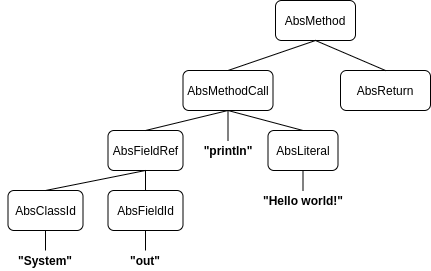
\includegraphics[width=12cm]{resource/HelloWorldAST.png}
\caption{Example abstract syntax tree for a simple \textit{"Hello world!"} program}
\end{figure}

\newpage
\subsection{UML Class Diagram}
The below UML class diagram simply shows the higher-level architecture of the compiler system. The entire program itself consists of 36 classes at the time of writing this report, which would render the showing of a full class diagram infeasible. Therefore notes are provided at the bottom of the diagram which detail the classes which did not appear as part of the class diagram.
\begin{figure}[H]
\centering
\includegraphics[width=\linewidth]{/home/luke/Pictures/classdiagram.png}
\caption{UML class diagram for Java compiler program showing higher level architecture}
\end{figure}
\newpage

\subsection{Running}
The below lines show how to run the compiler on some \texttt{/path/to/file.java} program after having cloned the repository.
\begin{verbatim}
git clone https://github.com/RHUL-CS-Projects/FullUnit_1920_LukeBessant
cd FullUnit_1920_LukeBessant/Java\ Compiler/bin
java -jar Java\ Compiler.jar /path/to/file.java
cd /path/to
java file.java
\end{verbatim}



















\newpage\section{Software Engineering}
\subsection{Version Control}
Over the course of the first term I used git as the version control system for my project, using my repository to store my research reports as well as proof of concept programs written and the final compiler product. The master branch was simply used to house releases of programs or reports, and was not used to develop on. The crux of the development was done on the dev branch, wherein both proof of concept programs and reports were edited. However predominantly the reports were updated through the docs branch before being merged to master. The final deliverable program, the Java compiler, was developed on its own compiler branch. Abiding to good version control practice, I frequently synced merge the development branches with master, and also merged these branches to master when some development milestone had been reached. 

I managed to maintain a consistent pattern of commits throughout the development of the programs, keeping up a good workflow and totalling at the point at which this report was written, 378 commits. This was due to commits being submitted whenever some \textit{business value} was added to the codebase, avoiding gargantuan additions of code.

\subsection{Documentation}
Javadoc was used to document the classes, fields and methods written across all of the proof of concept programs and the compiler product, which describes the purpose of each class or method in the program, and the purpose of and parameters used by methods in each program. Thus anyone with either of the programs is able to generate the javadoc pages for a given program, as well as understand the context of each component of the code. All of the programs within my project repository also have descriptions of how to run and use them, which will help people make use of my programs. Comments appear within the programs built wherever code written is ambiguous or difficult to understand at first glance.

\subsection{Testing}
Test-driven development was used during the development of most of the proof of concept programs, with the exception of the lexer generator, so that any bugs which could otherwise have been introduced into them were not produced.

\newpage\section{Conclusion}
Each of the proof of concept programs gave me some insight into the construction of components needed to build the final product of this project, being a compiler for a subset of Java. Key knowledge gained involves the specification of a context-free grammar for a language, the ability to build a lexer from a set of regular expressions corresponding to tokens, how to create and use abstract syntax trees and simple code generation. Therefore these proof of concept programs have been clear stepping stones towards the final deliverable, and have contributed to its design.

The final proof of concept program, the lexer generator, was one which did not appear in the initial project plan. This was originally a proposed final deliverable under the topic of computer language design and engineering on the project specification, however it seemed like a good way to learn more about recognition of strings as tokens in lexical analysis, therefore I chose this as an early deliverable.

The compiler product was, as expected, the most difficult program to implement. It required a wide range of skills, which although I could develop by making the proof of concept program, still required some practice and research. The byte code generation part of the program in particular required heavy research, since the code generation I had implemented for the calculator program was much simpler.


\newpage\part{Evaluation}

\section{Critical Analysis and Discussion}
\subsection{Achievements - Products}
The objectives and aims which I set out to achieve were on the most part very successful, with reports and programs written being submitted by the date first declared within my initial project plan. This showed that I maintained a good level of self discipline and professionalism, in that I was able to keep up with the academic punctuality levels I set out for myself. Having enjoyed this project from the get-go I put a lot of work into it, which produced the results I wanted to, as well as more. Following this is a list of particularly important objectives which stand out from the rest, and of which I was proud to complete. These contributed greatly to the advancement of my project.
%
\begin{itemize}
\item{\textbf{Report on context-free grammars:} My second report, this was my first real introduction into the intricacies of the compiler chain as my first report on interpretation versus compilation didn't go into great detail technically. Therefore this report was one of the key components in boosting my understanding of all things compilers, a stepping stone towards actually implementing a compiler.}

\item{\textbf{Report on lexical analysis:} This report was the next logical step following the report on context-free grammars, being the next stage to consider working up the compiler tool chain. In order to myself understand what goes on within the ANTLR parser generator, and perhaps even gain the ability to make my own lexer, it was necessary to produce this report.}

\item{\textbf{Report on top-down parsing:} Syntax analysis being the next stage in a compiler (generally) after lexical analysis, was another technology I had to get to grips with to understand how a compiler really works. I chose to concentrate the report on top-down parsing specifically due to ANTLR using the top-down \textit{LL(*)} algorithm in the parsers it produces. Furthermore as a reflection this report and those prior to this show my level of discipline to complete them and resourcefulness to go out and find the materials necessary to understand these technologies.}

\item{\textbf{Calculator interpreter program:} This was the second \textit{proof of concept} program I wrote during this project. Unlike the first program (the BNF pretty printer), this program required that I gain a much higher understanding of how to use abstract syntax trees; how one traverses them and simplifies them. This was relevant due to the need to look at a tree which corresponds to an input expression, and rewrite it in such a way that I could easily interpret the meaning behind the expression and consequently execute it to produce the correct result expected. 

This is a notable achievement because understanding how abstract syntax trees work is fundamental in implementing a compiler, since this is how the input program is represented after the parsing phase. This demonstrated to me that I had the ability to go on and perform more complex operations with these trees, such as the derivation of Java bytecode for my compiler product.}

\item{\textbf{Lexer Generator:} This program was an additional implementation which I did not assign to myself within the initial individual project plan. This was an additional objective added in during the first term due to progress being better than first thought in terms of implementation of proof of concept programs and report writing. The task was to implement a program which would take a regular expression and produce a minimal deterministic finite-state automaton representing it, which would accept strings belonging to the language of the expression; halfway to a full lexer generator program. I include this as a notable achievement because it proved that I was ahead of schedule with my project, that I could manage to fit in another program, arguably the most complex so far. This program also showed great understanding of how lexers work, and how to implement recognition of tokens.}

\item{\textbf{Java subset compiler:} This was the final product of my individual project which I was working up to implementing throughout the earlier stages of this process. Given all this, the fact that I have been able to implement a compiler which takes simple Java programs, produces an internal representation of such programs and generates a corresponding \textit{.class} file is, to me, the thing I am most proud of coming out of this project. It shows that all of the hard work researching and experimenting performed throughout the process has all been put to good use and has been well understood.

This product was a large project in itself and required a lot of understanding of the \textit{.class} file structure and the Java bytecode commands which I would need to use to perform actions synonymous to the desired effect intended in the input code. As well as this, I had to understand how code generation based off of a tree structure worked so that I could get to the point of being able to generate this output file. Consequently a lot of theoretical research as well as practical prowess were required to get this program to work properly, therefore rendering this product the greatest achievement of this project.} 
\end{itemize}
I believe that these achievements have demonstrated my competence in this field and have been executed in a way which allowed me to learn technologies that would be of great benefit in my final product.

\subsection{Achievements - Professionalism}
Acting professionally was also a key part of the individual project process, since demonstration of professionalism is one of the primary objectives of taking on an individual report in the first place; one can use their progress in this regard to improve their chances of obtaining the career they want. The major points of professionalism during the process of this project surround documentation of progress made along the way, as well as regular meetings with the project supervisor. The sort of documentation necesary includes diary entries, code commit comments and build instructions. 

In terms of meetings, I was able to maintain a regular schedule with my supervisor that included meetings every one or two weeks, depending on how much progress on a particular section of work was made. Therefore we met when there was some implementation or report to discuss, or any problems/issues arose. I believe that this was a good show of professionalism with regard to organisation, since my supervisor was kept up to date with the progress of my project. 

I also mostly maintained a good schedule of diary updates, involving progress made on the project and any problems encountered along the way. Diary entries were submitted at least once every week and were informative on work done since the last update. Consequently those overseeing my project were able to check in on my progress. In addition to this however, it allowed me to look back on the diary entries over the past terms and review the important stages, identifying problems I had and such.

Finally, I believe that the commit messages I uploaded whilst doing implementation were were also indicative of the work that I had put in, and inform the reviewers of the crux of the work done at each update of the repository. Again, this allows me and others to look back on the work and identify hurdles and achievements where and when they arose, giving this project a greater level of professionalism.

\subsection{Shortfalls}
\subsubsection{Implementation}
One of the main drawbacks of this review is the lack of time put into research on semantic analysis stage, and the \textit{back end} of general compilers; the optimisation and code generation stages. As a result of this, when it came to implementing these stages of the compiler I had to find out on the fly how to do things like type checking and code generation itself. This has lead to perhaps unconventional and deprecated means of completing these tasks due to the need to rush the research for these so that I could carry on with implementation and not get behind schedule with the implementation side of the project. 

Since having taken the course Software Language Engineering (CS3840) taught by Professor Adrian Johnstone, I now know I could have easily picked up on how to properly perform semantic analysis by reading the book for the course, \textit{Software Language Engineering}\cite{SLEBook}. I could have also read into code generation in \textit{Compilers: Principles Tools and Techniques}\cite{Dragon} (the dragon book) and the book \textit{Introduction to Compiler Design}\cite{ItCD}, which I own.

\subsubsection{Professionalism}
I mentioned previously that my diary entries for this project were, on the most part, informative and consistent. However there were still times when the diary entries I entered were lackluster, or irregular. These were times at which there were assignments present for other courses I took in both terms, however I should have been able to find time for my project daily, as was recommended when first starting this project. This was also synonymous with periods in which I wouldn't make any commits to any programs I was building, due to the commitment to other pieces of work set for me in other courses.

\subsection{Future Enhancements}
Improvements made in the future would primarily involve spending more time getting used to technologies and methods of implementation which are critical to the system I propose to build. I now have the benefit of knowing where pieces of knowledge are missing with regards to the general stages of the compiler chain, which will help me to implement similar such programs in the future. Not having to learn something like ANTLR trees on the fly will give me much more time to actually implement the program I'm working on. Perhaps also not having other courses to concentrate on will help me to put more time into research on the technologies I am looking to implement. This may also indicate that I should have put more time into the project than I had, whenever I had free time to do so, which is also another thing to consider next time.

With regards to professionalism I would also make improvements based on the drawbacks identified within the last section; firstly, I would maintain complete consistency in uploading diary entries and commits to my repository. This would also allow me to hold more regular meetings with my supervisor, since there would be more to talk about each time we met. In retrospect I would also organise my time in the week much better so that I had a time slot each day to which I allocated working on my project. Consequently I would make much more progress in implementing the set of features my programs need, allowing me to move onto further additional work.






\newpage\section{Technical Review}

\subsection{Project Scope}
I believe that from the outset of this project, its scope in terms of implementation was large enough to consume two terms full of work, but not too large to a degree where implementation was infeasible. Due to the tools and material available to me I was able to implement all of the programs I set out to complete, with time enough to allow me to work on further programs, which is how the lexer generator program came to be. None of the implementation necessary to complete the project programs which appeared in my project plan was too difficult to complete, however of course some of the technical details took much more thinking than others. I believe that, with the help of my project supervisor, I was able to overcome all of the implementation hurdles I came across, such as type checking for the compiler. Such hurdles are further described in section 15.4.

Specific to the compiler program, the original scope was to implement the ability for users to write their own classes, methods, and fields, as well as write some basic statements, expressions and control flow. With the exception of loops, all of these aims were achieved. Therefore I can conclude that the scope of the compiler was good, since implementation of loops is a simple step away and could have been achieved by submission were I not stuck on type checking for as long as I was.

\subsection{Use of Java}
I believe that using Java to implement the programs of this project was a good choice, since in the past I have had much experience in writing Java programs. This meant that I could build my programs without having to revise the basics of the language I was to be using. Furthermore, OpenJDK\cite{OpenJDK}, the compiler my operating system comes with, is also written in Java. Therefore we can declare that if Java is good enough for OpenJDK, it's good enough for us. Java being an object-oriented language also means that implementing the more modular parts of the compiler program was very straightforward. For example, the nodes of the abstract syntax tree can be easily implemented in a way that reduces the code we need to write for each node. This is because of object inheritance, which in one case was used for expression nodes, where the tree node for each type of expression inherited the ``parent" expression node.

\subsection{ANTLR Usage}
The ANTLR\cite{ANTLR} (v4) parser generator was used during the building of three of my four programs, the exception being the lexer generator proof of concept program. This was an important part of my implementations as it handled a large part of the work I would otherwise have had to do myself, that is, writing lexers and parsers for my context-free grammars. Therefore all of the work done between the initial running of the program and the first parse tree visit in each program is handled by ANTLR. This was extremely useful, as it meant I could concentrate on the ``back end" implementation of each program, for example, the type checking and code generation phases of my compiler program. 

I believe that the implementing of my own parser generator for this project would have itself taken a few months, which would have seriously limited the amount of time I had to work on the proof of concept programs and the compiler. Furthermore, the use of a widely popular parser generator almost guarantees that the lexing and parsing performed will be much more efficient than I could implement myself. This is because of many people having worked on it for a longer time than I have, which also decreases the risk of serious bugs coming impeding the development of my programs.

ANTLR uses a top-down \textit{LL} predictive parsing method with unlimited lookahead, denoted by \textit{LL(*)}, where the \textit{LL} stands for left to right input parsing and the constructing of a \textit{leftmost} derivation of an input. This method of parsing is one which does not suffer from having to backtrack, which results in faster and more efficient parsing. Due to this not being a \textit{general} parsing method, I had to write context-free grammars which do not include any left recursion, otherwise the parser would get stuck on rules which include this condition. This simply meant I had to be more careful when writing my grammars, and did not significantly impede my progress in any way. 

To conclude, using ANTLR was of great benefit to this project and allowed me to allocate the lexing and parsing stages to a well developed third-party toolset, whilst I could concentrate on the other more interesting phases of the compiler chain.

\subsection{Development Hurdles}
\subsubsection{DFA Minimisation}
This hurdle is concerned with the third proof of concept program, the lexer generator. The significant hurdle when writing this program was fixing the exponentially long running time of the powerset construction. At first without any optimisation, the generation of the DFA for the regular expression \texttt{[a-z][a-zA-Z0-9]*} took at least a minute. Clearly this could get much worse with DFAs which would require more states than this example, therefore this had to be fixed. At first this problem took a lot of head scratching, however my supervisor suggested the following resolution.

To fix this problem, instead of generating a whole DFA and then minimising the complete automaton, a minimal DFA was generated for each recursive step of Thompson's construction. This meant that at every point there was a kleene-closure (\texttt{a*} for some expression \texttt{a}), or alternation clause (\texttt{a|b} for some expressions \texttt{a},\texttt{b}), we minimise the clause as if it was a complete DFA. We then pass this minimal DFA up to the function which called the routine for this sub-expression. This may seem at first like a slow process since we're using both subset construction and hopcroft's minimisation algorithm for every sub-expression, however this provided much faster results than the minimisation strategy first used. This is because although we're running these algorithms more, the automata we use them on are significantly smaller.

\subsubsection{Type Checking}
The type checking problem was the second notable hurdle faced during the course of this project. The problem concerned wasn't due to complicated theory or misunderstanding of what type checking entails, since the sections of the books which detail type checking were fairly easy to understand. The problem was that I had hitherto built the compiler program without considering this essential topic, therefore when I got to the point of needing to derive the type of some field or method, I had no means with which to do so. This was silly on my part and showed some level of ignorance when I had to mend by reading up on type checking. 

The solution that presented itself was to implement some environment in which I could store the types of classes, fields and local variables, and which I could query for a type using the method/field/local variable's identifier. This also allowed me to implement variable scope later on. After having built this environment blueprint I found it easy to implement type checking within my compiler program, which opened the door to the work to follow, including assignment to variables and binary expressions.

\newpage\part{Bibliography}
\begin{thebibliography}{9}

\bibitem{ANTLR}
Parr, T. [\textit{ANTLR Parser Generator}] [\url{https://www.antlr.org/}]. 2014.

\bibitem{OpenJDK}
OpenJDK. [\textit{OpenJDK}] [\url{https://openjdk.java.net/}]. 2020.

\bibitem{Jikes}
Jikes. [\textit{Jikes}] [\url{http://jikes.sourceforge.net/}]. 2020.

\bibitem{GCJ}
Object Computing. [\textit{GCJ: The GNU Compiler for Java}] [\url{https://objectcomputing.com/resources/publications/sett/january-2003-gcj-the-gnu-compiler-for-java}]. 2020.

\bibitem{SLEBook}
Johnstone, A. Scott, E. [\textit{Software Language Engineering}]. 2019. 

\bibitem{Dragon} 
Aho, A. Lam, M. Sethi, R. Ullman, J.
[\textit{Compilers - Principles, Techniques, and Tools: Second Edition}]. 
2007.

\bibitem{ItCD}
Modensen, T. [\textit{Introduction to Compiler Design: Second Edition}] 2017.

\bibitem{HelloWorld}
Thomas, D. [\textit{Writing Hello World in Java Byte Code}] [\url{https://medium.com/@davethomas_9528/writing-hello-world-in-java-byte-code-34f75428e0ad}]. 2017

\bibitem{JavaToByteCode}
Bloom, J. [\textit{Java Code to Byte Code}] [\url{https://blog.jamesdbloom.com/JavaCodeToByteCode_PartOne.html}]. 2013.

\bibitem{ClassFile}
Oracle. [\textit{The Java Class File Format}] [\url{https://docs.oracle.com/javase/specs/jvms/se7/html/jvms-4.html}]. 

\bibitem{Crafting Interpreters}
Bob Nystrom [\textit{Crafting Interpreters}] [\url{https://www.craftinginterpreters.com/}]. 


\end{thebibliography}

\end{document}
